\documentclass[11pt,a4paper]{article}
\usepackage[left=2cm,text={17cm,24cm},top=3cm]{geometry}
\usepackage[T1]{fontenc}
\usepackage[czech]{babel}
\usepackage[utf8]{inputenc}
\usepackage{url}
\usepackage{graphicx}
\usepackage{pdfpages}
\graphicspath{ {img/} }

\begin{document}

\begin{center}
\LARGE{Administrátorské rozhraní pro CMS}
\end{center}
Číslo projektu: 1\\
Číslo a název týmu: 139. Tým xstehl14\\
Autor: Petr Stehlík (xstehl14) \\
Další členové týmu: Mário Kuka (xkukam00), Martin Veis (xveism00)\\
Termín řešení: 21. 9. - 18. 12. 2015\\


\section*{Abstrakt}
Administrátorská webová rozhraní trpí mnoha UX prohřešky. Majoritní většina je nepřátelská, nepomáhající a zmatečná. Je zde několik důvodů proč tomu tak je. Administrátoři jsou minoritní skupina uživatelů dané stránky, negenerují přímý zisk, ale zprostředkovaný, a v neposlední řadě u administrátorů je velká motivace dosáhnout cíle (většinou je jejich prací udělat na webu X a Y a pokud tuto práci neodvedou, nadřízený nebude spokojen).

Největším problém současných administrátorských rozhraní je naprostá oddělenost od uživatelské části. Administrátor se musí přihlásit na speciální stránce (každý systém má adresu této stránky jinou) a přes tu vstoupit do administrace. Na e-shopech, při editaci produktu, zde nejdříve musí vyhledat správnou část administrace, správnou kategorii, v horším případě vyhledat rovnou produkt mezi tisíci dalších a objeví se obrovský formulář pro editaci produktu.

S nastupujícími moderními technologiemi tento problém nemusí být až tak velký. Proto jsme se rozhodli navrhnout administrátorské rozhraní, které nebude až tak administrátorské jako spíše uživatelské. Administrátor nebude mít vlastní stránky na editaci, ale bude mít k dispozici editační mód přímo na stránce, kterou návštěvník vidí a použivá. Tím odpadá obrovská režie pro administrátora, který nemusí odhadovat, co uživatel uvidí, jak se změna projeví, atp. Své úpravy uvidí přímo na dané stránce v daný okamžik a tím se přibližíme k plně funčnímu WYSIWYG editoru.

\section*{Cílové požadavky na aplikaci a její rozhraní}
Hlavním cílem našeho snažení je vytvořit plnohodnotý e-shop, který nebude mít administrační rozhraní oddělené od uživatelského. Toho docílíme editačním módem uvnitř e-shopu. Aplikace tím pádem nemusí obhospodařovat dva, technicky vzato, rozdílné weby, ale vše obstará \uv{front-end} pro uživatele.

Odstraněním \uv{back-endu} dosáhneme rychlejší a smysluplné editace stránek. Administrátor není nucen přecházet mezi 2 stránkami a načítat celý obsah znovu. Jakoukoliv úpravu ihned vidí. To odstraňuje další problém rezonující napříč všemi e-shopy -- nevydařené úpravy. Uživatel nemůže přijít na e-shop, který je zrovna v údržbě.


\section*{Studium uživatelů, UI a testování}
Díky velmi specifické cílové skupině, pro kterou navrhujeme, jsou zde určitá omezení. Nemůžeme použít nepřesné nebo zavádějící názvy akcí. Na druhou stranu máme velmi motivovanou cílovou skupinu, která má jasné cíle. Touto problematikou se zajímá několik projektů, většina z nich je ale pouhým rozšířením stávajících CMS. Např. pro Wordpress existuje rozšíření Cornerstone\footnote{\url{http://www.liveeditorcms.com/}} nebo pro OpenCart Live Theme Editor\footnote{\url{http://www.opencart.com/index.php?route=extension/extension/info&extension_id=20693}}.

Nejefektivnější a nejvíce vypovídající metodologií testování je testování s reálnými uživateli. Např. A/B testování není v tuto chvíli proveditelné, protože nemáme zavedený eshop, na kterém bychom mohli testovat, navíc se jedná o kompletně nový CMS s vlastním databázovým schématem.


\section*{Návrh GUI}
Nejdůležitější funkčností aplikace je živá editace obsahu. Úpravy, které administrátor provede, okamžitě uvidí a může se tak rychle rozhodnout, zda úpravy, které provedl, jsou vhodné. Tímto způsobem může administrátor upravit jakoukoliv část webu a jeho obsahu, logem počínaje, patičkou konče.

Při návrhu GUI je vhodné používat interaktivní wireframe, protože v případě statických wireframe nedokážeme demonstrovat celkovou dynamičnost aplikace. Prvotní návrhy probíhají na papíře a ty přímo přetváříme do low-fidelity wireframe (viz Přílohy). Ten se následně vylepší a s dodanou funkcionalitou vytvoříme high-fidelity wireframe.

Po průzkumu současných e-shop CMS jsme zhodnotili, že tento typ rozhraní v současné chvíli neexistuje, případně jako pouhé pokusy. To s sebou nese řadu nevýhod, které ale eliminujeme nástroji odzkoušenými v praxi a zkušenostmi v oboru.

%%%%%%%%%%\Large{Připravte mockupy rozhraní}

\section*{Návrh testování}
Z hlediska povahy aplikace a jejího zaměření budeme provádět kvalitativní testování na několika typech uživatelů, kteří se s aplikací mohou dostat do styku. S ohledem na neveřejnost projektu by navíc bylo velmi těžké vytvořit kvantitativní testování.
\begin{enumerate}
	\item{Pokročilejší uživatelé PC}
	\item{Běžní uživatelé PC}
	\item{Počítačově negramotní uživatelé}
\end{enumerate}

Nejdůležitějšími skupinami uživatelů jsou číslo 1 a 2, kteří jsou nejpravděpodobnější uživatelé této aplikace. 

\section*{Studium realizace GUI}
Z hlediska povahy projektu je nejvhodnější webové řešení. Je zde i možnost desktopového řešení, ale tím by celý návrh ztratil smysl v podobě oddělénoho back-endu. Webové řešení má navíc několik výhod. Je velmi lehce přenositelné, dostupné kdekoliv (i na mobilních zařízeních) a nezávislé na platformě.

Nevýhodou webového řešení je částečně různá interpretace aplikace na různých webových jádrech prohlížečů. Tyto rozdíly jsou ale víceméně kosmetické a neubírají aplikaci na funkcionalitě.

Konkrétně pro front-end jsme vybrali velmi silnou kombinaci HTML 5 a CSS3 pro zobrazování a AngularJS\footnote{\url{https://angularjs.org/}} pro obsluhu front-endu. AngularJS je javascriptový MVC framework pro dynamickou manipulaci s webovou stránkou (pomocí two-way data binding). Zároveň slouží jako server pro celou stránku (z hlediska front-endu).

Pro serverový back-end jsme zvolili jazyk Python a knihovnu Flask\footnote{\url{http://flask.pocoo.org/}}. Back-end slouží pouze pro komunikaci s databází a kontrolu uživatelů (udržování session). Knihovna Flask je použita pro tvorbu webového API, aby mohl front-end komunikovat s back-endem. 

Python oproti PHP disponuje excelentní vyjadřovací schopností, je efektivnější a jednodušší k použití. Společně s různými knihovnami se tyto schopnosti ještě více umocňují.
% Jaké technologie jsou vhodné pro řešení aplikace a UI?
% Čím je vhodná vybraná technologie (Qt, WPF, web tech. apod.)? Co přináší a v čem je naopak takovéto řešení omezující?
% Jaké specifické části technologie (popř. rozšiřujících nástrojů) jsou pro řešení vybrány a proč?
% Sepište do TZ.

\section*{Návrh back-endu}
Pro plnou funkčnost aplikace je potřeba webový server s veřejnou IP adresou, v našem případě Linuxový server s Apache, databáze MySQL a jazyk Python s knihovnou Flask. Apache je konfigurován na spouštění WSGI skriptů (Python). 

Struktura celé aplikace je znázorněna na schématu, které ukazuje i použité technologie v jednotlivých částech aplikace.
\newline
\newline
\begin{figure}[ht]
\center
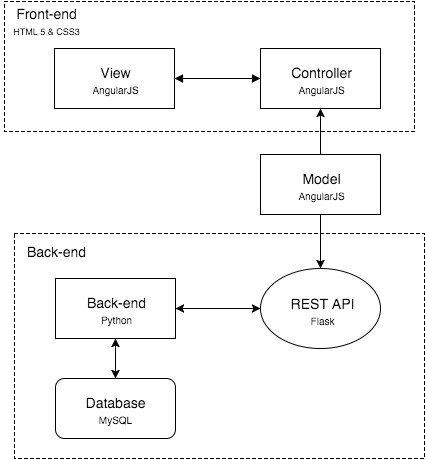
\includegraphics[scale=0.5]{schema.png}
\caption{Schéma aplikace}
\end{figure}

% Jaké služby/funkce (server, datový model, sada funkcí, služby třetích stran apod.) je třeba připravit pro dostatečnou funkčnost a testování GUI aplikace? 
% Funkce nemusí být funkční (dynamické apod.), ale musí vracet smysluplné hodnoty (simulované hodnoty, pevně přednastavené ...).
% Jaká je struktura aplikace a napojení GUI na back-end?
% Zpracujte do TZ.

% Programování back-endu
% Naprogramujte a připravte na použití. 
% Klíčové informace o back-endu (stručný popis, struktura programového řešení, vybrané funkce, API) popište v TZ.
% Toto nemusí dělat všichni členové týmu.

\section*{Programování back-endu}
Back-end je realizován v jazyku Python společně s knihovnou Flask. Ten obsluhuje veškerou práci s databází dle požadavků od front-endu. API je navrženo dle REST metodologie\cite{rest} s využitím CRUD\footnote{\url{http://www.infoworld.com/d/developer-world/rest-and-crud-impedance-mismatch-927}} operací.

\subsection*{Flask}
Flask je tzv. {\em microframework}, což v jednoduchosti znamená knihovnu, která je založena na několika dalších knihovnách, která dané frameworky spojuje a rozšiřuje jejich funkcionalitu. V případě knihovny Flask to jsou frameworky Werkzeug\footnote{\url{http://werkzeug.pocoo.org}} a Jinja 2\footnote{\url{http://jinja2.pocoo.org}}.

\subsubsection*{Werkzeug}
Werkzeug je WSGI knihovna pro zpracovávání HTTP požadavků a tím nahrazuje základní práce serveru (např. Apache nebo nginx). Díky této knihovně jsme schopni API provozovat na zvláštním portu, případně adrese, a kontrolovat kdo může do API přistoupit.

\subsubsection*{Jinja 2}
Jinja 2 v této aplikaci nepoužíváme, protože obstarává šablonovací systém podobně jako Latté pro PHP framework Nette. Pro šablony využíváme AngularJS a vlastní šablony napsané pomocí něj.

\subsection*{Databáze}
Databázové schéma bylo převzato z dřívějšího projektu do předmětu IDS z druhého ročníku. Toto schéma jsme upravili a rozšířili. Částečné schéma je níže v přílohách. Databázový systém jsme zvolili MySQL pro jeho rozšířenost a dobrou podporu mezi vývojáři.

\subsubsection*{MySQL konektor}
Abychom mohli provádět operaci s databází pomocí jazyka Python museli jsme vybrat knihovnu pro spojení Python a MySQL databáze. Zvolili jsme oficiální distribuci doporučenou na stránkách MySQL\footnote{\url{https://dev.mysql.com/doc/connector-python/en/}}


% Testování
% Proveďte testy a měření, proveďte sběr zpětných vazeb.
% Sepište do TZ.
% Tato kapitola může být částečně společná s dalšími členy týmu.

\section*{Testování}
Testování jsme prováděli na několika jedincích s různými znalostmi obsluhy počítače. Podle vytvořených scénářů uživatelů tvořili, editovali a spravovali systém, přičemž jsme je sledovali a poznamenávali si jejich postup. Ze získaných informací jsme usoudili následující:

\subsection*{Obecné závěry}
Pro všechny skupiny uživatelů bylo v prvních momentech práce se stránkou nezvyklá absence administrační části aplikace. To ale brzy pochopili a velice rychle adaptovali své chování jiné logice systému.

Další nezvyklost byla editace textu přímo ve stránce, největší problém jsme identifikovali v potvrzení editace textu, kdy kliknutím mimo textovou oblast se text neuloží a zůstane původní. Pro uložení textu je potřeba potvrzení tlačítkem {\em SAVE}. Toto lze vyřešit automatickým ukládáním textu.

\begin{figure}[h]
    \centering
    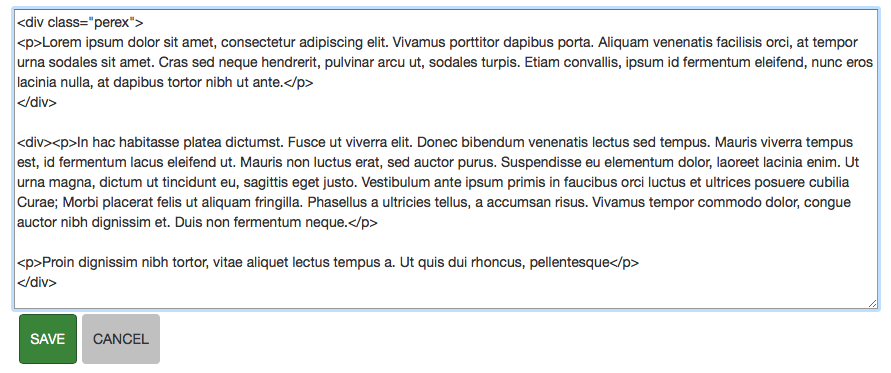
\includegraphics[width=\textwidth]{edit.png}
    \caption{Editace textů produktu}
\end{figure}

\subsection*{Méně zkušení uživatelé}
Lidé se základní uživatelskou znalostí obsluhy počítače měli v prvních momentech se systém spíše logický problém, protože nejsou zvyklí na okamžité projevy úprav na stránce. Vždy čekali zda se stránka znova načte, což v našem případě není nutné.

\subsection*{Zkušenější uživatelé}
Administrátoři dalších e-shopů neměli s úkony téměř žádný problém, adaptace na jinou logiku systému editace stránek byla relativně rychlá a bez komplikací.

\section*{Výsledky a závěr}
% Zpracujte výsledky testů.
% Jaké jsou závěry z naměřených a zpracovaných výsledků?
% Jaké postupy/prvky zafungovaly? Jaké naopak nefungují dle očekávání?
% Výsledky diskutujte.
% Tato kapitola může být částečně společná s dalšími členy týmu.
Při testu jsme měřili za jaký čas uživatelů zvládnout daný úkol. Před testováním jsme odhadli nejdelší čas, ve kterém bz uživatel dokázal úkol provést bez pocitu frustrace.

\subsection*{Test č. 1 -- Vytvořte nový produkt v kategorii XYZ}
Uživatelé měli za úkol vytvořit nový produkt v dané kategorii. Kategorii jsme zadávali jak v první úrovni, tak v kategorii vnořené. Z výsledků usuzujeme, že uživatelé neměli pocit frustrace a uživatelský zážitek byl veskrze kladný.

\begin{figure}[ht]
    \centering
    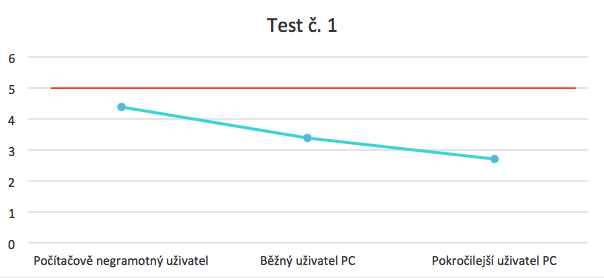
\includegraphics[width=\textwidth]{t1.png}
    \caption{Vytvoření nového produktu}
\end{figure}

\subsection*{Test č. 2 -- Upravte produkt ABC v kategorii XYZ}
Úkolem bylo nalezení produktu v dané kategorii a jeho editace. Jelikož šlo o druhý pokus v řadě uživatelé již pochopili logiku prostředí a výsledné vnímání prostředí bylo kladné, pouze nezkušení uživatelé mírně tápali.

\begin{figure}[t]
    \centering
    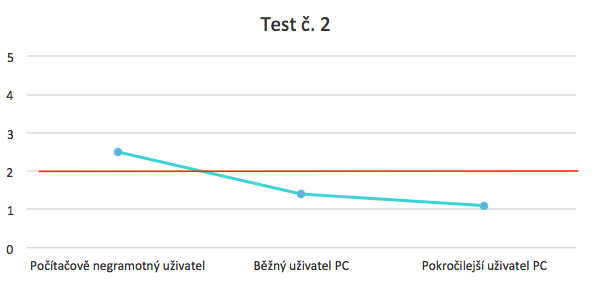
\includegraphics[width=\textwidth]{t2.png}
    \caption{Editace textů produktu}
\end{figure}

\subsection*{Test č. 3 -- Vyřiďte příchozí objednávky (vytisknout faktury)}
Jediný test, který neproběhl dle našich předpokladů. Uživatelé nevěděli kde přesně nálezt objednávky a následně hledali funkci vytisknout všechny faktury. Pro jednoduchost aplikace jsme nezaváděli funkci uložit do PDF, protože současné prohlížeče umožňují danou stránku uložit jako PDF. Takto jsme koncipovali tuto funkcionalitu. Pro lepší zážitek je vhodné akce pojmenovat lépe.

\begin{figure}[!ht]
    \centering
    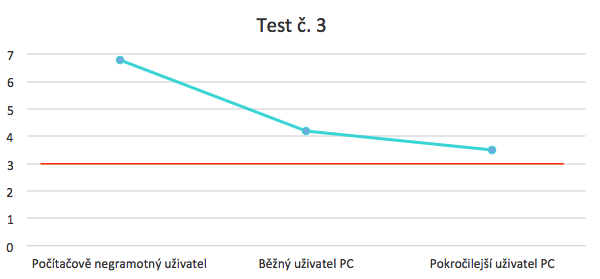
\includegraphics[width=\textwidth]{t3.png}
    \caption{Vytisknutí faktur}
\end{figure}
\newpage

\subsection*{Test č. 4 -- Upravte název kategorie A na B}
Nejrychlejší a nejjednodušší úkol ze všech. Nepředpokládali jsme žádné komplikace a úsudek byl korektní. Editace proběhla bez problémů.

\begin{figure}[!ht]
    \centering
    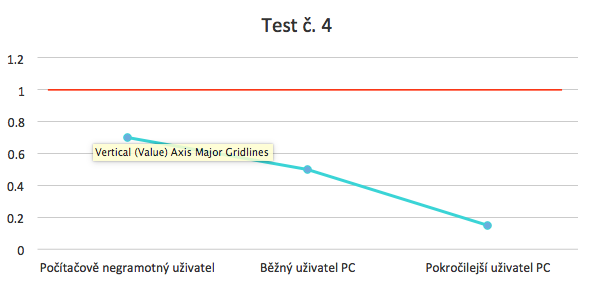
\includegraphics[width=\textwidth]{t4.png}
    \caption{Upravení názvu vnořené kategorie}
\end{figure}


Můžeme konstatovat, že prostředí je uživatelsky přívětivé a snadné k použití. Občas se vyskytly drobné chyby, které ale nikterak dramaticky nesnižují uživatelský zážitek. Při pohledu na výsledky vidíme, že i nezkušení uživatelé se rychle adaptovali a úkoly nebyly pro ně složité či frustrující. Z testování jsme si odnesli důležité poznatky jak prostředí vylepšit.


\section*{Týmová spolupráce}
% Stručně reflektujte, co Vám přinesla možnost pracovat na projektu ve více lidech a v čem byla naopak spolupráce omezující.
% Sepište pouze pokud jste pracovali v týmu.
Práce v týmu pro nás byla bez větších komplikací, protože náš tým již pracoval ve stejném složení na předchozích projektech. Věděli jsme co jeden od druhého očekávat a jaké množství práce je schopen odvést. Novinkou pro nás bylo zavedení systému git\cite{git} (konkrétně služby GitHub), kterou jsme částečně používali v předchozích projektech, ale tento projekt byl kompletně celý spravován přes systém git.


\section*{Závěr}
% Shrnutí cílů, postupu a dosažených výsledků.
Cílem projektu bylo vytvoření administrační části CMS. Naše řešení je rozdílné v tom, že administrační část je spojena s uživatelskou a tím pádem jsme museli vytvořit obě části. Pro naše řešení jsme zvolili exotické a moderní technologie, se kterými jsme dosáhli kvalitních výsledků. Podařilo se nám vytvořit prostředí, které je uživatelsky přívětivé, rychlé a snadné na obsluhu. Celé řešení je plně funkční a přenositelné na jakýkoliv webový server.


\begin{thebibliography}{1}

  \bibitem{rest} Richardson, Leonard; Sam Ruby {\em  RESTful web service} 2007, ISBN 978-0-596-52926-0.
  \bibitem{git} Chacon, Scott {\em Pro Git} 2014, ISBN 978-1-484-20077-3

\end{thebibliography}

\section*{Přílohy}

\subsection*{Návrh rozhraní -- běžný uživatel}
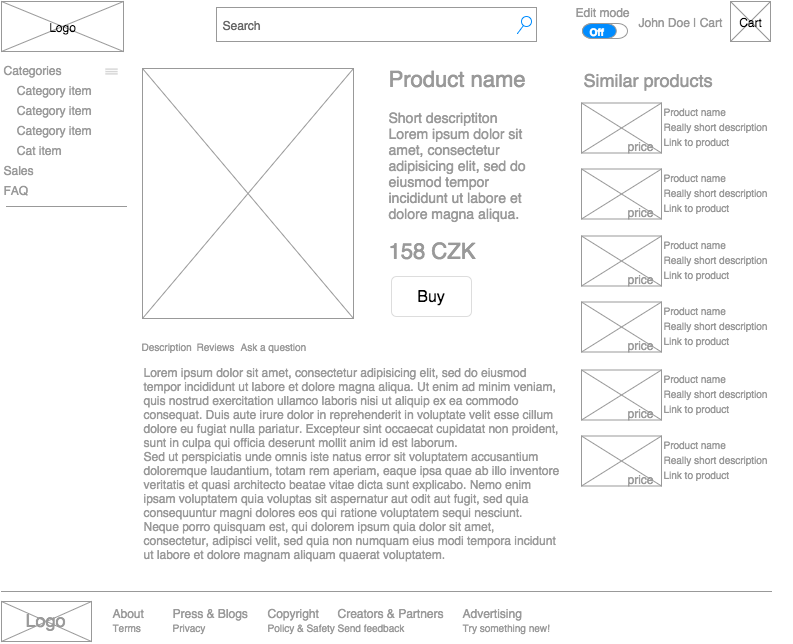
\includegraphics[scale=0.6]{pyngshop.png}
\subsection*{Návrh rozhraní -- administrátor}
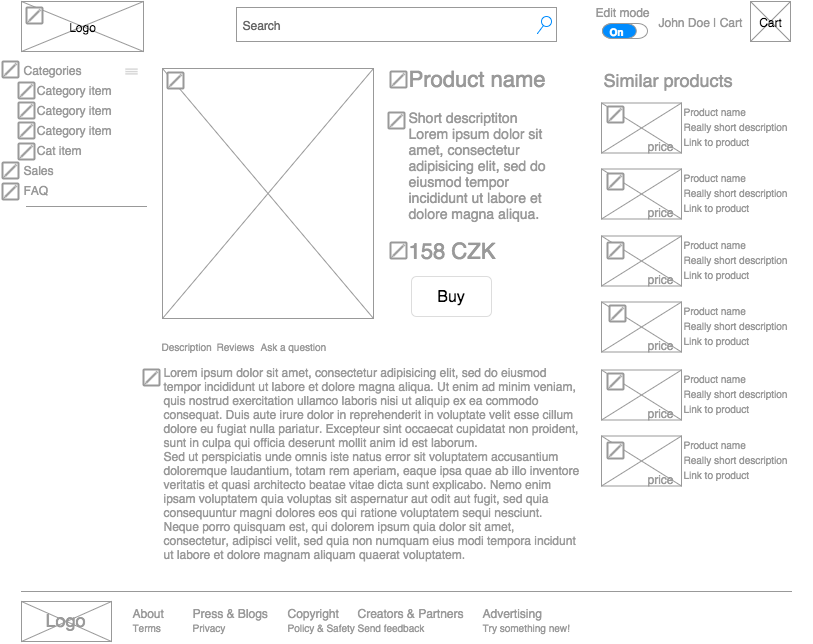
\includegraphics[scale=0.6]{pyngshop_edit.png}
\newpage

\subsection*{Databázové schéma}
\centerline{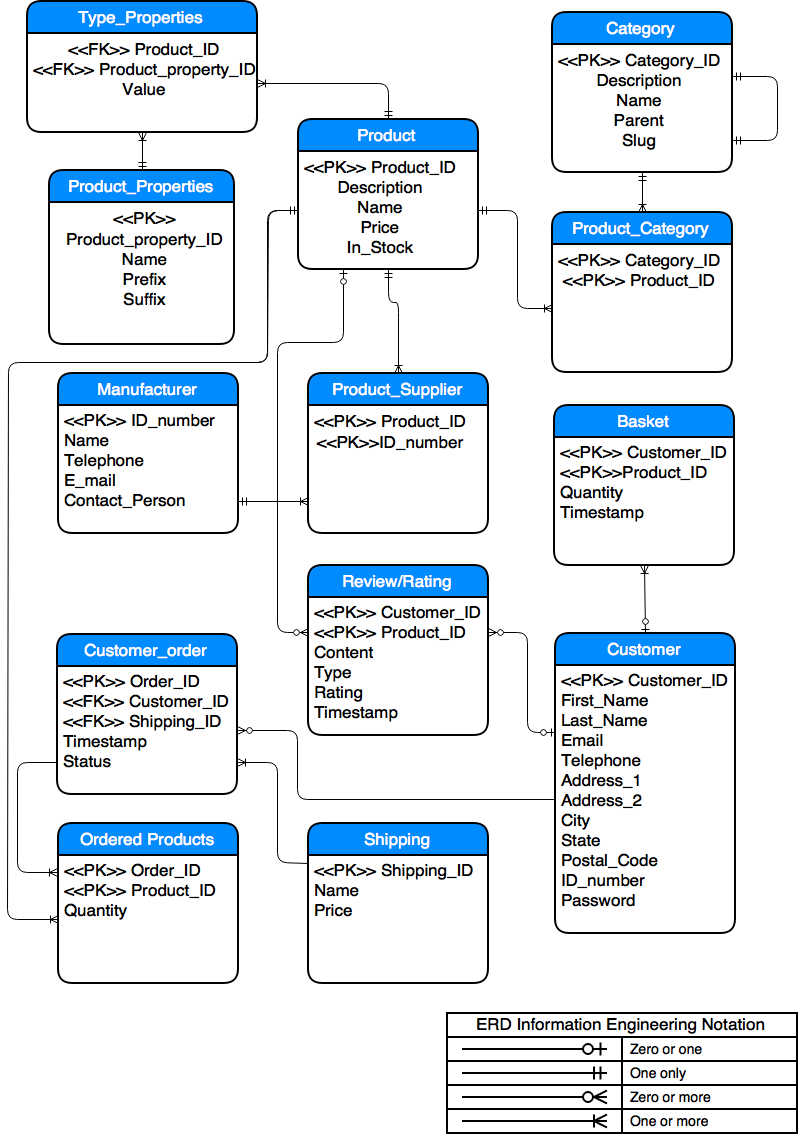
\includegraphics[scale=0.55]{eshop_erd.png}}
\newpage

\subsection*{Testovací protokol}
\noindent{\large\textsc{Úkol}: Vytvořte nový produkt v kategorii XYZ.}\\
\textsc{Cíl}: Vytvoření produktu v dané kategorii.\\
\textsc{Čas}: 5 minut s připravenými podklady.\\
\bigskip

\noindent{\large\textsc{Úkol}: Upravte produkt ABC v kategorii XYZ.}\\
\textsc{Cíl}: Upravení produktu v dané kategorii.\\
\textsc{Čas}: 2 minuty pro minoritní úpravu.\\
\bigskip

\noindent{\large\textsc{Úkol}: Vyřiďte příchozí objednávky (vytisknout faktury).}\\
\textsc{Cíl}: Vytištění faktur do PDF a uložení.\\
\textsc{Čas}: 3 minuty do finálního uložení všech faktur.\\
\bigskip

\noindent{\large\textsc{Úkol}: Upravte název kategorie A na B.}\\
\textsc{Cíl}: Upravení názvu zanořené kategorie.\\
\textsc{Čas}: 1 minuta.\\
\bigskip

\noindent Ke každému úkolu zaznamenáváme čas provedení, komplikace při provádění, otázky uživatele, úroveň frustrace vykonavatele, úroveň zmatení a spokojenost s výsledkem


<<<<<<< HEAD
\end{document}
=======
\end{document}
>>>>>>> 9ff189f... ADD: final docs
